\chapter{Quality Assurance}
\label{vl:tc-QA}

\section{Overview of DUNE Quality Assurance}

\dshort{dune} \dword{tc} monitors technical contributions from
collaborating institutions and provides centralized project
coordination functions. One part of this project coordination is
standardizing \dfirst{qa}/\dfirst{qc} practices, one facet
of which is to assist consortia in defining and implementing
\dword{qa}/\dword{qc} plans that maintain uniform, high
standards across the entire detector construction
effort. Figure~\ref{fig:fnal_qa} shows how \dword{dune} \dword{tc}
derives its \dword{qa} program from the principles of the \fnal \dword{qa} program:
requirements are flowed down through the \dword{lbnf-dune}
\dword{qa} Program into the \dword{qc} plans developed for consortia fabrication of
detector components and integration and installation of the detector.
\begin{dunefigure}[\fnal QA]{fig:fnal_qa}
  {Flow-down of \fnal \dword{qa} to consortia}
  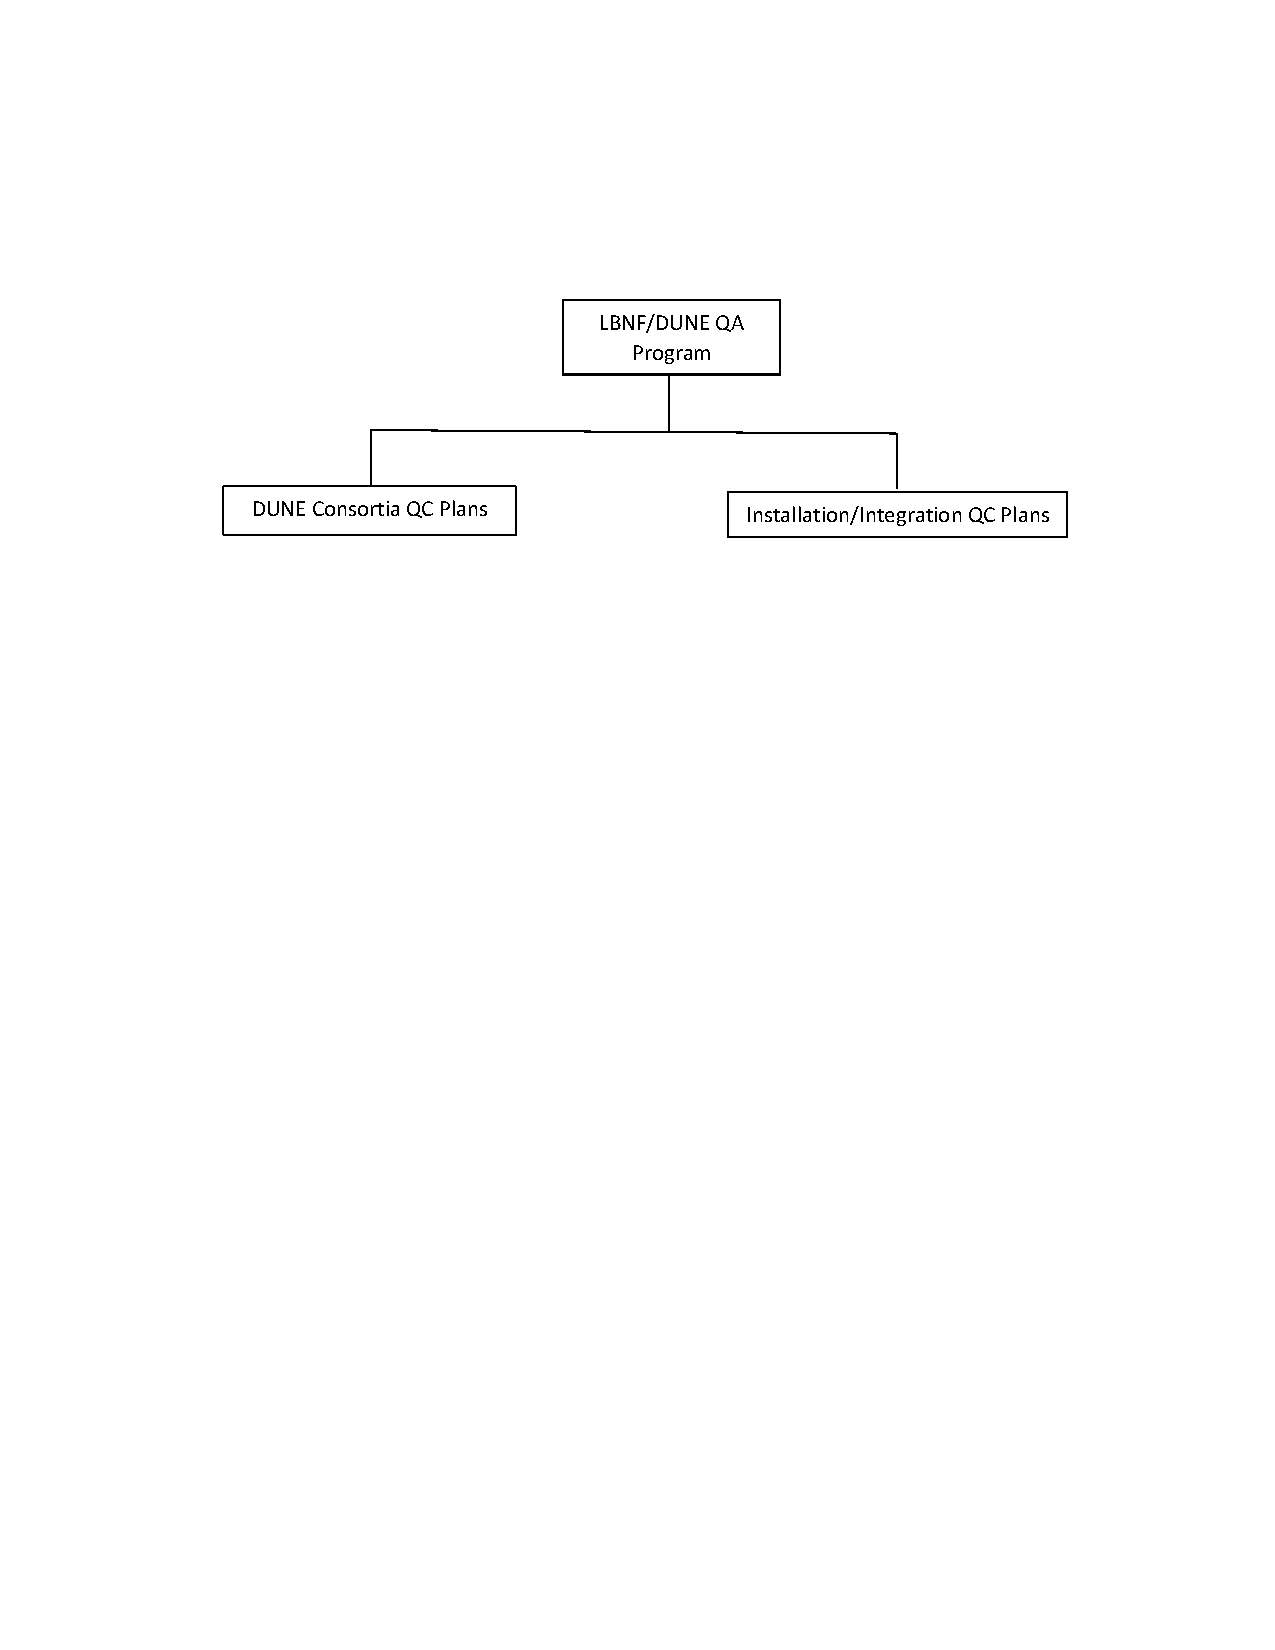
\includegraphics[width=0.85\textwidth]{fnal_qa.pdf}
\end{dunefigure}
The \dword{qa} effort includes design, production readiness and
progress reviews as appropriate for the \dword{dune} detector
subsystems as was done for \dword{pdsp} under \dword{tc}
oversight. Installation and operations reviews fall under \dword{jpo}
oversight.

\subsection{Purpose}

The primary objective of the \dword{lbnf-dune} \dword{qa} program is
to assure quality in the construction of the \dword{lbnf} facility and
\dword{dune} experiment while providing protection of
\dword{lbnf-dune} personnel, the public and the environment. The
\dword{qa} plan aligns \dword{lbnf-dune} \dword{qa} activities, which
are spread around the world, with the principles of the \fnal Quality
Assurance Manual. The Manual identifies the \fnal Integrated Quality
Assurance Program features that serve as the basis for the
\dword{lbnf-dune} \dword{qa} plan.

The \dword{lbnf-dune} \dword{qa} plan outlines the \dword{qa}
requirements for all \dword{lbnf-dune} collaborators and
subcontractors and describes how the requirements shall be met.
\Dword{qa} criteria can be satisfied using a graded approach. This
\dword{qa} plan is implemented by the development of quality plans,
procedures and guides by the consortia to accommodate those specific
quality requirements.

\subsection{Scope}

The \dword{lbnf-dune} \dword{qa} plan provides \Dword{qa}
requirements applicable to all consortia, encompassing all activities
performed from research and development (R\&D) through fabrication and
component commissioning, building on the success of
ProtoDUNE. Consortia are responsible for providing their deliverables,
whether subsystems, components or services in accordance with
applicable agreements. All parties are responsible for
implementing a quality plan that meet the requirements of the
\dword{lbnf-dune} \dword{qa} plan. Oversight of the work of
the consortia will be the responsibility of the \dword{dune}
\dword{tcoord} and \dword{lbnf-dune} \dword{qa}
manager.

\subsection{Graded Approach}

A key element of the \dword{lbnf-dune} \dword{qa} plan is the
concept of graded approach; that is, applying a level of analysis,
controls and documentation commensurate with the potential for an
environmental, safety, health, or quality impact. The graded approach
seeks to tailor the kinds and extent of quality controls applied in
the process of fulfilling requirements. Application of the graded
approach entails:
\begin{itemize}
  \item Identifying activities that present significant \dword{esh}
    and/or quality risk
  \item Defining the activity
  \item Evaluating risk and control choice
  \item Documenting and approving the application of the graded
    approach.
\end{itemize}

\section{Quality Assurance Program}

The \dword{lbnf-dune} Systems Engineering teams maintain a
\dword{lbnf-dune} \dword{cmp}, which identifies the \dword{lbnf} project
Configuration Items Data List (CIDL) and Interface Control matrices
that provide the tier structure for the flow down of \dword{qa} plans,
with the \dword{lbnf-dune} \dword{qa} plan as the top tier.

Specific \dword{qa} plans shall be developed by the consortia with the
assistance of the \dword{lbnf-dune} \dword{qa} manager for
component or system quality assurance. Due to the limited scope of
work of some consortia, they may elect to work under the
\dword{lbnf-dune} \dword{qa} plan for their scope of work. In
case of conflict between sets of \dword{qa} requirements, \dword{dune}
\dword{tc} will provide resolution.

With many institutions carrying responsibility for various aspects of
the project, institutional \dword{qa} plans will be reviewed by
\dword{dune} \dword{tc} to ensure compliance with the
\dword{lbnf-dune} \dword{qa} plan. Using a graded approach,
supplements to institutions existing plans will be implemented for
their \dword{dune} scope of work, if necessary.

Overall \dword{qa} supervision, including all activities described
above, is the responsibility of the \dword{dune} \dword{tcoord}.

\subsection{Responsibility for Project Management}

The \dword{dune} consortia leaders manage their projects and are
responsible for achieving performance goals. The
\dword{lbnf-dune} \dword{qa} manager is responsible for
ensuring that a quality system is established, implemented and
maintained in accordance with requirements. The
\dword{lbnf-dune} \dword{qa} manager reports to the
\dword{dune} \dword{tcoord} and provides oversight and support to
consortia leaders to ensure a consistent quality program.

\dword{dune} consortia leaders are responsible for quality within
their project and report Quality Assurance issues to the \dword{dune}
\dword{tcoord} and \dword{lbnf-dune} \dword{qa}
manager. \dword{dune} consortia leaders designate \dword{qa}
representatives within their organization and delegate, as appropriate, 
work defined in the \dword{lbnf-dune} \dword{qa} plan, as
shown in Fig.~\ref{fig:dune_qa}.
\begin{dunefigure}[DUNE QA organization]{fig:dune_qa}
  {\dword{dune} \dword{qa} organization}
  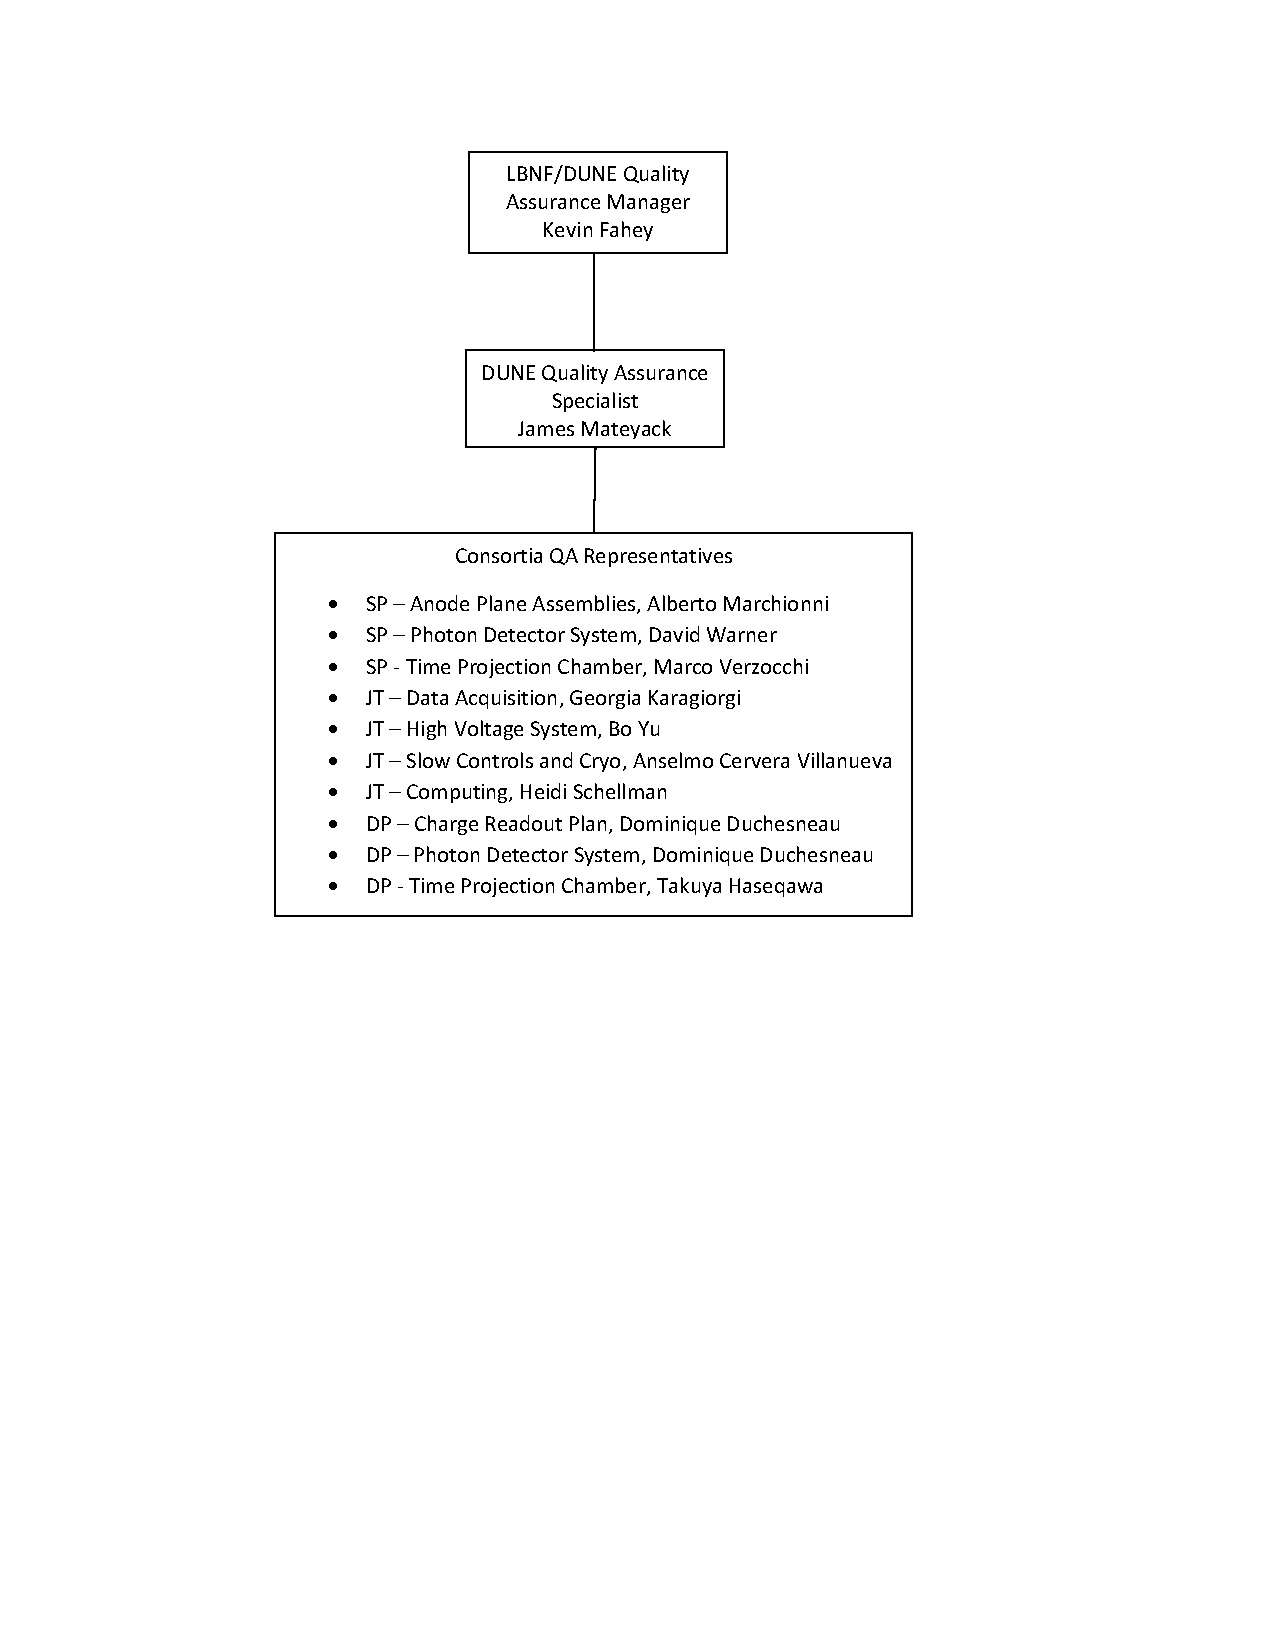
\includegraphics[width=0.75\textwidth]{dune_qa.pdf}
\end{dunefigure}
The \dword{dune} consortia leaders retain overall responsibility for
\dword{qa} even though they have designated a \dword{qa}
representative.

\subsection{Levels of Authority and Interface}

The \dword{dune} Management Plan, the \dword{lbnf-dune} PMP
and the \dword{lbnf-dune} \dword{qa} plan define the
responsibility, authority and interrelation of personnel who manage,
perform and verify work that affects quality. The \dword{qa} plan
defines the \dword{qa} roles and responsibilities of the \dword{dune}
project.

All consortia members are responsible for the quality of the work that
they do and for using guidance and assistance that is available. Each
has the authority to stop work and report adverse conditions that
affect quality of \dword{dune} products to their respective
\dword{dune} consortium leader and the \dword{lbnf-dune}
\dword{qa} manager. The consortium leader responsible for \dword{dune}
components or systems is required to determine and document their
acceptance criteria. \dword{dune} personnel at each level are
responsible for evaluation of quality through self-assessments;
however, independent quality assessments may also be requested by
project management.  The \dword{lbnf-dune} \dword{qa} manager is
responsible for development, implementation, assessment and
improvement of the \dword{qa} program.

The \dword{lbnf-dune} \dword{qa} manager is responsible for
periodically reporting on the performance of the quality system to the
\dword{dune} \dword{tcoord} for review and as a basis for improving
the quality system. The \dword{dune} \dword{tcoord} may call for
\dword{qa} plan readiness assessments as the project nears major
milestones. The \dword{dune} \dword{tcoord}, consortia leaders and
\dword{lbnf-dune} \dword{qa} manager are all responsible for
providing the resources needed to conduct the project successfully,
including those required to manage, perform and verify work that
affects quality.

\subsection{Quality Assurance Organization}

\dword{lbnf-dune} \dword{qa} manager may request personnel
from the \dword{dune} project to act on behalf of the
\dword{lbnf-dune} \dword{qa} manager to perform quality
assurance functions, based on need, in accordance with the graded
approach described above. The requested personnel shall possess
qualifications or receive the appropriate training required to perform
these functions.

The \dword{dune} \dword{qa} Specialist will be responsible for the
following activities:
\begin{itemize}
	\item Cooperatively develop, monitor and control \dword{dune}
          \dword{qa} procedures to assure compliance with \dword{dune}
          standards and applicable laws
     \item Provide assistance for \dword{qa}/QC matters in project
       plans, including strategizing technical solutions and
       alternatives on \dword{qa}/QC matters and assist in developing
       testing plans with project team members
	   \item Participate in audits, site inspections, accident
             investigations, and monitor trend analysis to identify
             areas of concern and implement improvements
	\item Interact with all stakeholders on \dword{qa} issues
      \item Provide guidance and interpretation on routine and complex
        \dword{qa} matters and problems
	\item Participate in reviews at collaborating institutions
\end{itemize}

Each consortia selects a \dword{qa} Representative for the consortia.  The
Quality Assurance Representative is responsible for overall
coordination of quality requirements to assure they meet consortia
objectives.  The \dword{qa} Representative responsibilities include:
\begin{itemize}
  \item Oversee the consortia fabrication facilities for quality
    performance
  \item Interface with the DUNE \dword{qa} Specialist on consortia \dword{qa} related
    matters
  \item Monitor the status of all required testing based on the
    consortia QC Plan
  \item Make sufficient fabrication facility visits to determine
    adequacy of QC System performance, such as: Check certifications
    of materials and equipment delivered to the facility, spot check
    workmanship, observe testing procedures
  \item Make or arrange \dwords{ppr} during the fabrication cycle in
    coordination with \dword{tc}
\end{itemize}

Figure~\ref{fig:dune_qa} shows the interface between the
\dword{lbnf-dune} \dword{qa} organization and the consortia \dword{qa}
Representatives.
These interfaces will remain when the equipment is shipped to the far
site for installation, but the names may change for the consortia \dword{qa}
Representatives.  The consortia \dword{qa} Representatives remain responsible
for \dword{qa}/QC during the detector installation process.


\section{Personnel Training and Qualification}

The \dword{dune} consortia leaders are responsible for identifying the
resources to ensure that their team members are adequately trained and
qualified to perform their assigned work. Before allowing personnel to
work independently, they are responsible to ensure that their team
members have the necessary experience, knowledge, skills and
abilities. Personnel qualifications are based on the following
factors:
\begin{itemize}
 \item previous experience, education and training
 \item performance demonstrations or tests to verify previously
   acquired skills
 \item completion of training or qualification programs
 \item on-the-job training
\end{itemize}

All \dword{dune} consortia leaders are responsible for ensuring that
their training and qualification requirements are fulfilled, including
periodic re-training to maintain proficiency and qualifications.


\section{Quality Improvement and Lessons Learned}
\label{sec:quality_improvement}

All \dword{dune} consortia members participate in quality improvement
activities that identify opportunities for improvement. They can
respond to the discovery of quality-related issues and follow up on
any required actions. This quality-improvement process requires that
any failures and non-conformance be identified and reported to the
appropriate consortia leader; and, that root causes be identified and
corrected. All consortia members are encouraged to identify problems
or potential quality improvements and may do so without fear of
reprisal or recrimination. Items, services and processes that do not
conform to specified requirements shall be identified and controlled
to prevent their unintended use. Inspection and test reports or
similar tools will be used to implement this requirement. Each
consortia leader is responsible for reporting non-conformance to the
\dword{lbnf-dune} \dword{qa} manager and the
\dword{lbnf-dune} \dword{qa} manager will periodically report
these non-conformance to \dword{dune} \dword{tc}.

\dword{dune} consortia members will perform Root Cause Analysis and
Corrective and Preventive Actions for conditions that do not meet
defined requirements. Consortia leaders may perform Root Cause
analysis and Corrective and Preventive Actions under their own
procedures or \fnal procedures.  This problem identification, analysis
and resolution process for quality consists of the following steps:
\begin{enumerate}
  \item Identify problem
  \item Understand the process
  \item Grade the process and identify Root Cause Analysis (RCA)
    method
  \item Identify possible causes
  \item Collect and analyze data
  \item Communicate Lessons Learned and document RCA
  \item Implement Corrective and Preventative Action procedure
\end{enumerate}

%\subsection{Lessons Learned}  this was a single subsection within a section
%\label{sec:lessons_learned}

To promote continuous improvement, \dword{dune} \dword{tc} will develop a
lesson learned program based on the \fnal Office of Project Support
Services Lessons Learned Program. This program provides a systematic
approach to identify and analyze relevant information for both good
and adverse work practices that can influence project execution. Where
appropriate, improvement actions are taken to either promote the
repeated application of a positive lesson learned or prevent
recurrence of a negative lesson learned. Lessons learned shall be
gathered throughout the project life cycle. As part of the transition
to operations a lessons learned report will be submitted.

In addition, the \dword{lbnf-dune} \dword{qa} manager will
periodically publish a best practices and lessons learned
report. Lessons learned from the \dword{dune} project will be screened
for applicability to other organizations. The \dword{dune} project
will periodically check external lessons learned sources for
applicability to the \dword{dune} project. Sources of lessons learned
include the \dword{doe} Lessons Learned List Server, the \fnal \dword{esh}
Lessons Learned Database, and \dword{dune} team members who
participate in peer reviews of other projects. Reviews of the
\dword{dune} project serve as input to quality improvement.

\section{Documents and Records}

Engineering and scientific documents (including drawings) are prepared
by \dword{dune} personnel to define the design, manufacture and
construction. Ultimately, before these documents are put into effect
they are reviewed and signed by the \dword{dune} consortia leader or
designee. \fixme{all scientific documents cannot be correct.} The
\dword{dune} project manages all documents under the document control
systems: \dword{edms} and \docdb, as identified in the \dword{dune}
\dword{cmp}.  The system to control document preparation, approval,
issuance to users and revision is described in the CMP. Consortia
leaders will use the graded approach described in this plan to
determine work in their scope that requires the \dword{lbnf-dune}
\dword{qa} manager review and signature. Project documents that
contain quality requirements shall be reviewed by the
\dword{lbnf-dune} \dword{qa} manager.

Records are prepared and maintained to document how decisions are
made, for instance, decisions on how to arrive at a design, how to
record the processes followed to manufacture components and the means
and methods of cost and schedule change
control. \dword{lbnf-dune} will follow the guidelines for
storing and maintaining records for the project in accordance with
\fnal Records Management(http://ccd.fnal.gov/records). The
\dword{dune} \dword{tcoord}, \dword{lbnf-dune} \dword{qa}
manager and consortia leaders are responsible for identifying the
information to be preserved. In addition to the technical, cost and
schedule baseline and all changes to it, records must be preserved as
evidence that a decision was made or an action taken and to provide
the justification for the decision or action.

\section{Work Processes}

\dword{dune} team members are responsible for the quality of their
work, and consortia leaders are responsible for procuring the
resources and support systems to enable their staff to complete their
work with high quality. All \dword{dune} work will be performed using
methods that promote successful completion of tasks, conformance to
\dword{dune} requirements and compliance with the
\dword{lbnf-dune} \dword{ieshp}. Work processes consist of a
series of actions planned and carried out by qualified personnel using
approved procedures, instructions and equipment, under administrative,
technical and environmental controls, to achieve a high-quality
result.

\subsection{Fabrication Work Processes}

Fabrication work on the \dword{dune} project shall be performed to
established technical standards and administrative controls using
approved instructions and procedures. Fabrication work processes with
\dword{qa} inspections and tests shall be documented on Travelers that
are retained with the hardware item. Items, including consumables,
shall be identified and controlled to ensure their proper use and
prevent the use of incorrect, unaccepted or unidentified items. The
consortia will define a system of controls to ensure that items are
handled, stored, shipped, cleaned and preserved to prevent them from
deteriorating, being damaged or becoming lost. Equipment used for
process monitoring or data collection shall be calibrated and
maintained.

Work shall be performed safely, in a manner that ensures adequate
protection for employees, the public and the environment. Consortia
members and the \dword{dune} \dword{tcoord} shall exercise a degree of
care commensurate with the work and the associated hazards. See the
\dword{lbnf-dune} \dword{ieshp} for more details on
\dword{lbnf-dune} integrated safety management systems.

\subsection{Change-Controlled Work Processes}

Changes to design and fabrication requirements should follow the normal 
revision process for design and fabrication documents ensuring the 
appropriate level of verification, review and approval by the consortia 
and \dword{tc}.


When shop or site work must be performed before the affected design 
document can be formally revised and re-issued such changes are 
accomplished through the development, approval and distribution of an 
Engineering Change Request (ECR). This process is for designs that are 
under configuration management. Interdisciplinary reviews shall be 
performed when the ECR subject matter may impact other disciplines. The 
Design Authority shall indicate if it is a one-time change or if the 
change shall be incorporated into the design documents.

\section{Design}

The \dword{dune} design process provides appropriate control of design
inputs and design products. The primary design inputs are the
\dword{dune} scientific/engineering requirements (physics
requirements, detector requirements, specifications, drawings,
engineering reports, etc.) as discussed in
Section~\ref{sec:fdsp-coord-requirements}.

The basis of the design process requires sound engineering judgment
and practices, adherence to scientific principles, and use of
applicable orders, codes and standards. This basis of the design
process naturally incorporates environment, health and safety
concerns.

\subsection{Design Process}

The \dword{lbnf-dune} Systems Engineering website
documentation defines the scope of design work for any given
scientific/engineering work group. From this source, work groups
will begin preliminary design of \dword{dune} by breaking their work
down into sets of engineering drawings, specifications and
reports. This is the design output.

Throughout the design process, engineers and designers work with
consortia leaders and the \dword{lbnf-dune} \dword{qa} manager to
determine \dword{qa} inspection criteria of fabricated products and
installations. Close coordination must be made with \dword{dune}
scientists to assure the engineering satisfies the scientific
requirements of the experiment. Configuration Management as documented
in the \dword{lbnf-dune} \dword{cmp} will be
systematically implemented for \dword{dune}. Final Design work sets
the final Quality Assurance parameters for the parts, assemblies and
installations. Design during Final Design and production is confined
to Change-Controlled changes, as above; and, minor changes necessary
to facilitate production, drawing error correction, material
substitutions and similar functional areas.

\subsection{Design Verification and Validation}
\label{sec:verification}

Design is verified and validated to an extent commensurate with its
importance to safety, complexity of design, degree of standardization,
state of the art and similarity to proven design
approaches. Acceptable verification methods include but are not
limited to any one or combination of (1) design reviews, (2)
alternative calculations, and (3) prototype, qualification testing
and/or (4) comparison of the new design with a similar proven design
if available. Verification work shall be completed before approval and
implementation of the design.

Design reviews shall verify and validate that the following criteria
are met at the appropriate milestone:
\begin{itemize}
 \item Adherence to requirements
 \item Technical adequacy of the design
 \item Adequacy of work instructions
 \item Thoroughness of specifications
 \item Test results
 \item Adequacy of Technical Reports
 \item Adequacy of design calculations and drawings
 \item Reliability and maintainability
 \item Calibration program for measurement and test equipment
\end{itemize}
The \dword{dune} Review Plan as discussed in
Chapter~\ref{vl:tc-review} describes the design reviews recommended
for its consortia.

Wherever the design method involves the use of
computer software to make engineering calculations or static dynamic
models of the structure, system, or component's functionality, the
software must be verified to demonstrate that the software produces
valid results. The verification needs to be documented in a formal
Report of Validation that is maintained in records that are accessible
for inspection. However, exemptions may be made for commercially
available software that is widely used and for codes with an extensive
history of refinement and use by multiple institutions. Exemptions
affecting systems or components shall be identified to the
\dword{lbnf-dune} Systems Engineering team.

Critical software and firmware computer codes, especially those codes
that are involved in controlling \dword{dune} data acquisitions
systems (DAQ), shall also be subjected to reviews for verification and
validation. Some items to be considered during computer code review
are as follows:
\begin{itemize}
\item Adequacy of code testing scheme
\item Code release control and configuration management
  \item Output data verification against code configuration
  \item Verification that code meets applicable standards `
  \item Verification of code compatibility to other systems that use
    the data
  \item Verification that code meets applicable hardware requirements
  \item Adequacy of code maintenance plans
  \item Adequacy of code and data backup systems
\end{itemize}

Validation ensures that any given design product conforms to \dword{dune}
requirements.
During reviews, validation of conformity to requirements
follows verification that the engineering design or computer code
meets all criteria. Engineering designs and computer codes shall be
validated, preferably before procurement, manufacture, or
construction; but no later than acceptance and use of the item; this
is to ensure the design or computer code:
\begin{itemize}
 \item Meets \dword{dune} requirements
 \item Contains or makes reference to acceptance criteria
 \item Identifies all characteristics crucial to the safe and proper
   use of the equipment or system and its associated interfaces
\end{itemize}

Each inspection, test or review will feed the \dword{qa} evaluation
process, which is a comparison of results with acceptance criteria to
determine acceptance or rejection. Rejection identifies the need for
Quality Improvement based on Section~\ref{sec:quality_improvement}. In
some cases, the outcome of the Quality Improvement process may be to
request change(s) to the design requirements.

\dword{qa} reporting formality escalates as the significance of the
inspection, test or review nonconformance increases. Higher levels of
management must be aware of and participate in the correction of the
most significant nonconformance. Section~\ref{sec:quality_improvement}
identifies the required course of action when nonconformance is
encountered.

\section{Procurement}

\subsection{Procurement Controls}

\fixme{Don't we need a Fabrication Controls section? that includes
  acceptance criteria for deliverabes? And non-corfmance exceptions by
  TC.}  Procurement controls will be implemented to ensure that
purchased items and services meet \dword{dune} requirements and comply
with the \dword{lbnf-dune} \dword{qa} plan.  The consortia members
requesting procurement of items and services are responsible for
providing all documentation that adequately describes the item or
service being procured so that the supplier can understand what is
required for consortia acceptance. Development of this documentation
may be achieved through the involvement of consortia Leaders and
established review and approval systems. The following factors will be
considered for review and approval of this documentation:
\begin{itemize}
 \item Inclusion of technical performance requirements
 \item Identification of required codes and standards, laws and
   regulations
 \item Inclusion of acceptance criteria, including requirements for
   receiving inspection and/or source inspection
 \item \dword{dune} requirements for vendor qualifications and
   certifications
 \item \dword{dune} intention to perform acceptance sampling in lieu
   of full inspection and test item acceptance
\end{itemize}
NOTE: For Vendor Qualification and acceptance of purchased items or
material by consortia members this may be performed under their own
institution requirements.

Previously accepted Suppliers shall be monitored to ensure that they
continue supplying acceptable items and services. Source surveillance
is the recommended method to ensure that items are free of damage and
that specified requirements are met. Supplier deliveries will be
verified against previously established acceptance criteria.

Unacceptable supplier items or services shall be documented. Records
of supplier performance, Inspection Test Records (ITR) and
contract-required submittals, are kept for future procurement
consideration.

Inspections shall be conducted to detect counterfeit and/or suspect
parts. For work funded by \dword{doe}, when counterfeit/suspect parts
are found, they will be identified, segregated and disposed of in
accordance with the \fnal Quality Assurance Manual Chapter 12020
Suspect/Counterfeit Items (S/CI) Program. \dword{dune} consortia may
use their own institutional procedure for counterfeit/suspect parts.

\subsection{Inspection and Acceptance Testing}

Inspection and testing of electrical, mechanical and structural
components, associated services, and processes by consortia members
shall be conducted using acceptance and performance criteria. ITR
forms, Travelers, and a Traveler database are the primary tools used
to organize this activity. Inspections will be conducted in accordance
with the graded approach.

Once equipment is received at the warehouse at SURF, the equipment will 
be inspected for shipping damage and accuracy against the Bill of Lading. 
Consortia members will perform any additional inspection and testing that 
is required by their design documents either at the warehouse or 
underground in the clean room as the equipment is prepared for 
installation.

Equipment used for all inspections and tests shall be calibrated and
maintained. Calibration will be controlled by a system or systems
making appropriate use of qualified calibration service
providers. Consortia Leaders shall ensure that equipment requiring
calibration have their calibration status identified on the item or
container, are traceable back to the calibration documentation and are
tracked to ensure the equipment is calibrated at the required
interval. The \dword{lbnf-dune} \dword{qa} manager shall
oversee and support the \dword{dune} calibration programs.

\section{Assessments}

\subsection{Management Assessments}

\dword{dune} management at all levels shall regularly evaluate
achievement of personnel relative to performance requirements and
shall appropriately validate or update performance requirements and
expectations to ensure quality of products and processes. The
management assessment process shall periodically include an evaluation
of the consortia products and processes to determine whether the
project's missions are being fulfilled. The results of management
assessments that focus on means of improving the quality of work
performed shall be reported to the appropriate responsible line or
project management level.

When performance does not meet established standards, management
shall, with the assistance of others with appropriate expertise,
determine the cause and initiate corrective action. \dword{qa}
representatives may assist, lead or facilitate cause investigations.

\subsection{Independent Assessments}

The \dword{lbnf-dune} \dword{qa} manager will plan reviews as
independent assessments to assist the \dword{dune} \dword{tcoord} in
identifying opportunities for quality/performance-based improvement
and to ensure compliance with specified requirements. Independent
assessments of the \dword{dune} projects can be requested by
\dword{dune} management. Independent assessments typically focus on
quality or \dword{esh} management systems, self-assessment programs, or
other organizational functions identified by management. The
\dword{dune} project uses a formal process for assigning
responsibility in response to recommendations from independent
assessments. These recommendations are tracked to closure.

Personnel conducting independent assessments shall be technically
qualified and knowledgeable in the areas assessed. A qualified lead
assessor (auditor), who is a Subject Matter Expert (SME) in the
technical area of assessment, is required. The team may include other
SMEs to evaluate the adequacy and effectiveness of activities only if
they are not responsible for the work being assessed.

The \fnal Directorate appoints an independent Long Baseline Neutrino
Committee (LBNC) to advise it and \dword{dune} Management. The role of
this standing committee is described in the \dword{lbnf-dune}
PMP. The \dword{doe} and other funding agencies perform external
assessments that provide an objective view of performance and thus
contribute to the independent assessment process. Since such
assessments are not under the control of \dword{dune}, they are not
necessarily considered a part of the independent assessment
criterion. However, \dword{dune} management considers external
assessment results in determining the scope and schedule of
independent assessments.

\section{ProtoDUNE to DUNE QA Approach}

The approach to \dfirst{qa}/\dfirst{qc} for \dword{dune} is going to be
very similar to the activities and oversight that was performed for
\dword{protodune}.  For \dword{protodune}, the major
\dword{qa}/\dword{qc} activities included review of consortia
\dword{tdr} \dword{qa}/\dword{qc} Sections; assisting the consortia in
development and review of \dword{qc} Plans (Production and
Installation), fabrication, inspection and test procedures,
installation plans and documentation; and the performance of
\dword{prr} at eleven consortia fabrication facilities.  There was
also \dword{qa} participation in the \dword{protodune} Design Reviews.
The \dword{prr} looked at the following criteria:
\begin{itemize}
  \item Final \dword{qa} plans for institutions not adopting the
    \dword{lbnf-dune} \dword{qa} Plan
  \item Final production drawings, specifications and manufacturing
    and test procedures
  \item Final safety documents (i.e., Hazard Analysis documentation
  \item Component \dword{qc} plan (i.e., travelers, test reports,
    software verification and validation documents, supplier
    documentation)
  \item Final procurement documents per institution practice
  \item Completion and evaluation of prototypes, review of production
    process and \dword{qc} results
\end{itemize}
The reviews ensured the facilities
were prepared for production and any kinks in the processes had been
identified and mitigations have taken place. The positive outcome of
these reviews was the amount of equipment received at CERN with little
to no damage.

\dword{ppr} will be performed at the fabrication facilities for the
\dword{dune} detector components. The review has been added due to the
larger number of components required and the increased number of
fabrication facilities. The goal of these reviews is to ensure
consistent fabrication processes between the facilities. If an issue
is identified at one facility it can be communicated to the other
applicable facilities to prevent the same issue occurring.

For \dword{protodune}, installation was performed at CERN under the
guidance of CERN policies and procedures. Installation of the
\dword{dune} detector at \dword{surf} will fall under similar procedures in the
\dword{lbnf-dune} \dword{qa} plan.
